\section{Interactions and vibrational spectra}

Spectroscopy is the field of science which studies the interactions between electromagnetic radiation and matter~\cite{kecki}. In general, processes of interest could be divided into two groups: absorption or emission of the radiation. The vibrational spectrum is related to changes in vibrational energy states during interaction of the studied system with radiation. It is observed in the energy range corresponding to the differences between the vibrational energy levels, commonly expressed in units of cm$^{-1}$, i.e. between 10~and 12~000~cm$^{-1}$. The basic techniques in vibrational spectroscopy are infrared (IR) spectroscopy and Raman spectroscopy.

Selection rules for vibrational spectroscopy are the following:
\begin{itemize}
    \item the energy of the photon must match the difference between two vibrational states:
    \begin{equation}
        \Delta E = h \nu
    \end{equation}
    \item non-zero change of the vibrational quantum number $v$: $\Delta v = \pm 1, \pm 2, \pm 3, ...$
    \item non-zero intensity $I$ of the band, for IR spectroscopy intensity $I_{\text{IR}}$ is proportional to change of the dipole moment during changing normal coordinate:
    \begin{equation}
    I_{\text{IR}} \sim \left| \left( \frac{\text{d} \mu}{\text{d} q} \right)_{q = q_e} \right|^2,
    \label{eq:ir-proportion}
    \end{equation}
    while for the Raman spectroscopy it is related to polarizability:
    \begin{equation}
        I_{\text{Raman}} \sim \left| \left( \frac{\text{d} \alpha}{\text{d} q} \right)_{q = q_e} \right|^2,
    \end{equation}
    where $q_e$ stands for the equilibrium position of the normal coordinate $q$.
\end{itemize}

The potential energy of a~vibration $U$, could be expressed as Taylor series around the equlibrium position $q_e$:
\begin{equation}
    U(q) = U(q_e) + \frac{1}{2} \kappa (q - q_e)^2 + \mathcal{O}(q^3),
    \label{eq:potential-energy-vibration}
\end{equation}
where $\kappa$ stands for the force constant of the vibration and is defined as follows:
\begin{equation}
    \kappa = \left( \frac{\partial^2 U}{\partial q^2}\right)_{q = q_e}.
\end{equation}

Retaining only terms up to $q^2$ in the equation~\ref{eq:potential-energy-vibration} corresponds to a~commonly used harmonic oscillator approximation. For a~vibration, the $\kappa$ value characterizes the strength of the oscillator, e.g., the strength of the particular bond. It can be calculated by standard quantum chemical methods by determining the second derivatives of the energy. In the harmonic oscillator appproximation, it is related to the vibration frequency $\nu$ by the formula:
\begin{equation}
    \nu = \frac{1}{2\pi} \sqrt{\frac{\kappa}{\mu_{\text{red}}}},
\end{equation}
where $\mu_{\text{red}}$ is the reduced mass of the oscillating system.

Many types of chemical bonds have visible bands in the IR spectrum in a~specific range of frequency, e.g. C=O stretching vibration usually appears between 1600 and 1750~cm$^{-1}$~\cite{sadlej-spektroskopia}. For this reason, IR spectroscopy is commonly used especially in organic chemistry, to identify functional groups present in the studied sample~\cite{clayden-t1}.

Interactions influence the potential energy surfaces, therefore, vibrational spectroscopies (IR or Raman)  could be used to detect and to study interactions in the system. The blue shift or the red shift of a~particular band with change of some conditions may suggest an increase or decrease of the bond strength. Appearance of a~new band could be a~result of new intermolecular interaction, e.g. when comparing the spectrum of neat solvent and a~salt solution. It is a~common situation when hydrogen bonds (HBs) are present. For example, an effect of competition between molecules could be observed, e.g. when hydrogen bonding is possible both as a~solvent-solvent or solvent-solute substance interaction. It should be noted that complexes formed by these interactions must have a long enough lifetime to be observed in the IR spectrum, i.e. this lifetime is larger than the period of interacting electromagnetic wave, which for IR is equal about $10^{-13}$~s~\cite{kecki}.

\begin{figure}
    \centering
    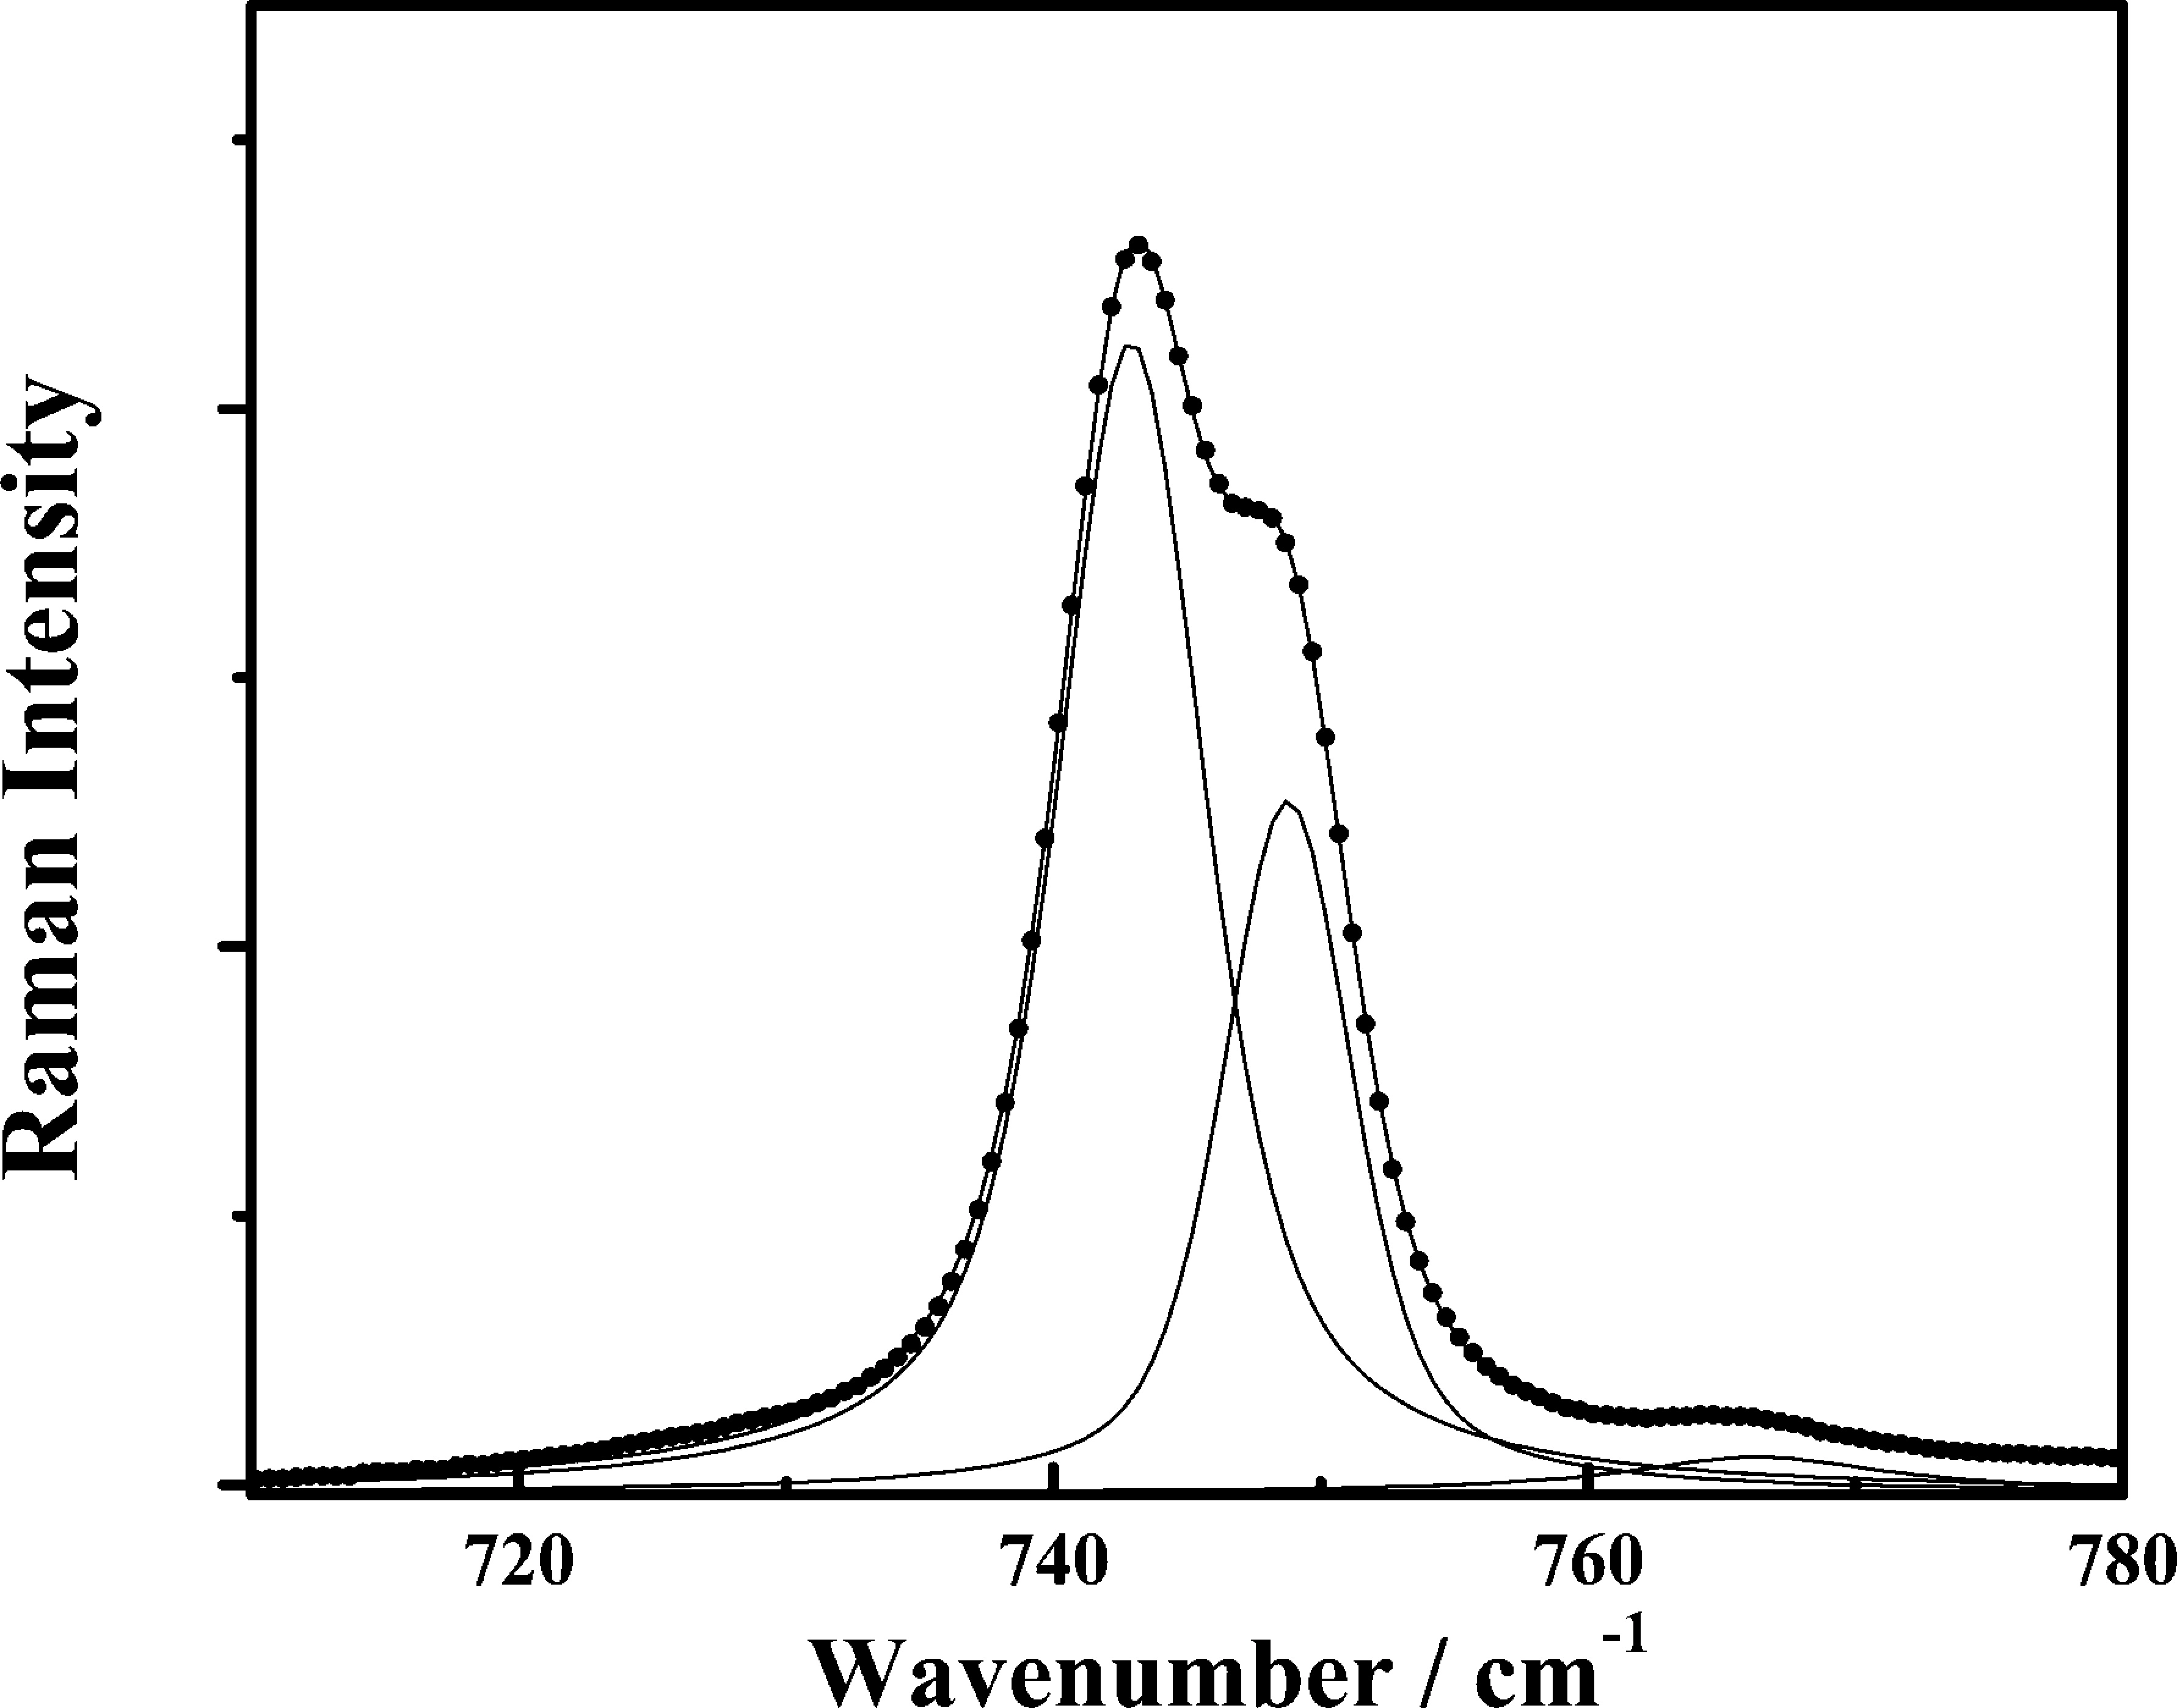
\includegraphics[width=0.75\textwidth]{img/1-introduction/ir-interactions-example.png}
    \caption[Raman spectrum of EMIM-TFSI solution with dissolved LiTFSI~\cite{li-interactions-4}]{Raman spectrum of EMIM-TFSI solution with dissolved LiTFSI. Dotted line is the experimental spectrum and the solid lines are the deconvoluted bands for free TFSI$^{-}$ (744 cm$^{-1}$), bound TFSI$^{-}$ (750 cm$^{-1}$) and EMIM$^{+}$ (766 cm$^{-1}$)~\cite{li-interactions-4}}
    \label{fig:1-ir-interactions-example}
\end{figure}

In the literature, there are many examples of studies of interaction through vibrational spectroscopy. One class of them is related to the strength of interactions. For example, IR spectra were used to study the solvent effect in nitriles~\cite{ir-interactions-10}, or for ionic liquids (ILs), which are a~part of interest in this work, like for monitoring the state of protonation of the anion~\cite{ir-interactions-11} or the strength of interations between ions in ILs based on imidazolium derivatives~\cite{ir-interactions-12}. Such spectra are able to study changes in the chemical environment. Due to their sensitivity to these differences, some molecules containing interaction-sensitive groups are proposed as probes. For example, in the ILs mentioned, benzonitrile was used as a~probe of the chemical environment due to the high sensitivity of the CN stretching vibration in the nitrile group~\cite{ir-interactions-13}. Similarly, the thiocyanate group has been presented as an analogous probe for proteins~\cite{ir-interactions-14}. The study of interactions by vibrational spectroscopy is also used for biological systems, for example, to examine interactions between carbohydrates and dried proteins~\cite{ir-interactions-1}, between alginate and chitosan biopolymers~\cite{ir-interactions-6} or adsorption abilities of humic acid on different nanosized media~\cite{ir-interactions-7}.

Another class of works utilizes vibrational spectra in verification of hypotheses about system structures. Symmetry-related selection rules for vibrational spectra allowed the identification of stable conformers, their populations, and their thermal dependence in systems studied in this work such as 1,2-dimethoxyethane~\cite{raman-interactions-1}, 1-ethyl-3-methylimidazolium bis(fluorosulfonyl) imide (EMIM-FSI)~\cite{raman-interactions-2} or glymes~\cite{raman-interactions-3}. For other systems, this symmetry effect was used to identify structures of benzenesulfonate complexes~\cite{ir-interactions-3}, propose structure of poly(\textsc{l}-lactic acid) crystals~\cite{ir-interactions-8} or to determine the structure of cathinone derivatives complexes~\cite{ir-interactions-4}.

Vibrational spectroscopy is also a~sensitive tool to study hydrogen bonds (HBs)~\cite{ir-interactions-15}. There are some articles describing HBs in ILs, which are most of the systems studied in this work. IR spectroscopy, along with other experimental methods, was used for determination of HB strength in a~set of ILs~\cite{ir-interactions-18,ir-interactions-16}. Other work described the low-frequency part of the spectrum for ILs contaminated with water~\cite{ir-interactions-17}. Raman spectra were used to study the formation of HB in ILs by monitoring shifts of the C=O, C=C and NH$_2$ stretching modes~\cite{raman-interactions-4}. Such studies are not limited to ILs; for example, research on HB formation was done for N-methylacetamide mixtures with water~\cite{ir-interactions-2} as well as for mixtures of water and heavy water~\cite{ir-interactions-5}. 

In further parts, this work concentrates on liquid systems that could be used as electrolytes for batteries, which were also studied by vibrational spectroscopy. Since the technology of lithium-based batteries is known for a~long time, there are many works that describe the properties of such systems. Raman spectra were used for the identification of Li$^{+}$ coordination in LiClO$_4$ solutions in ethylene carbonate (EC) and its derivatives~\cite{li-interactions-1,li-interactions-2} and it was observed that the bands related mainly to C=O stretching and ring deformation are influenced by increasing the concentration of the salt. In the systems based on gamma-butyrolactone and dimethylformamide, Li$^{+}$ coordination to carbonyl group was proved by IR measurements~\cite{li-interactions-3}. For a~system based on ionic liquid --- ethyl-3-methylimidazolium bis(trifluoromethanesulfonyl) imide (EMIM-TFSI), analysis of intensity changes revealed that the lithium cation has coordination number equal~4 and is coordinated by oxygen atoms from two TFSI$^{-}$ anions~\cite{li-interactions-4}. A~sample spectrum and its deconvolution is shown in the Figure~\ref{fig:1-ir-interactions-example}: a~new band corresponding to the TFSI$^{-}$ anions interacting with the Li$^{+}$ cations is readily visible. Analogous results were obtained for systems with different imidazolium derivative as cation~\cite{li-interactions-7}, systems based on LiBF$_4$~\cite{li-interactions-8} or LiPF$_6$~\cite{li-interactions-9} salt, systems with polyester-based polymer~\cite{li-interactions-5} or LiTFSI solutions in different solvents~\cite{li-interactions-6}. Another work shows that in concentrated LiTFSI solutions in ionic liquids, the lithium coordination number becomes less than~2 and aggregate formation is possible~\cite{lib-vibrational-modeling,li-interactions-10}. IR spectroscopy was used to study the changes in the lithium ion coordination scheme at different temperatures~\cite{li-interactions-11}.

Vibrational spectroscopy was also utilized to study interactions in novel electrolytes for metal-ion batteries, i.e. those based on other cations than lithium --- usually sodium. Similarly to lithium-based electrolytes, systems containing polymers such as poly(ethylene oxide) (PEO) were studied, and Raman spectroscopy results indicated that in the system containing NaFSI salt more anions are coordinated to the cation compared to the electrolyte with NaTFSI salt~\cite{ir-interactions-9}. For systems based on ionic liquids, the dependence of band positions in the Raman spectrum on NaTFSI concentration has been determined~\cite{na-il-5}. A~similar study was performed for glyme-based systems~\cite{na-interactions-1}.